\documentclass[12pt, a4paper]{article}
\usepackage[margin=1in] {geometry}
\usepackage{booktabs}
\usepackage{diagbox}
\usepackage{graphicx}
\usepackage{ragged2e}
\usepackage{tabularx}
\usepackage{fancyhdr}
\usepackage{palatino}
\usepackage{tikz}
\usepackage{amsthm}
\usepackage{leftidx}
\usepackage{latexsym}
\usepackage{titlesec}
\usepackage{mathptmx}
\usepackage[normalem]{ulem}
\setcounter{secnumdepth}{4}
\usetikzlibrary{shapes.geometric, arrows}

\parindent 0pt
\parskip 5pt
\pagestyle{fancy}

\fancyhead[L]{Consensus}
\fancyhead[R]{COMP90020 Distributed Algorithms}
\fancyfoot[L]{Semester 1, 2020}
\fancyfoot[C]{}
\fancyfoot[R]{\thepage}
\fancypagestyle{firststyle}{%
  \fancyhf{}
  \fancyfoot[L]{Semester 1, 2020}
  \fancyfoot[R]{\thepage}
  \renewcommand{\headrulewidth}{0pt}
}
\renewcommand{\headrulewidth}{0.4pt}
\renewcommand{\footrulewidth}{0.4pt}

\title{\textsc{Consensus}}
\author{
  Qifan Deng \\
  \texttt{\small qifand@student.unimelb.edu.au}
  \and
  Zhaofeng Qiu \\
  \texttt{\small zhaofengq@student.unimelb.edu.au}
  \and
  Alan Ung \\
  \texttt{\small alanu@student.unimelb.edu.au}
  \and
  Yangzhe Xie \\
  \texttt{\small yangzhex@student.unimelb.edu.au}
  \and
  Min Zhao \\
  \texttt{\small zhaomz1@student.unimelb.edu.au}
}
\date{Semester 1, 2020}

\newtheorem*{assumption*}{\assumptionnumber}
\providecommand{\assumptionnumber}{}
\makeatletter
\newenvironment{assumption}[2]
 {
  \renewcommand{\assumptionnumber}{Assumption #1}
  \begin{assumption*}K
  \protected@edef\@currentlabel{#1}
 }
 {
  \end{assumption*}
 }
\makeatother
\newcommand{\asref}[2]{\ref{#1}}

% https://tex.stackexchange.com/questions/60209
\titleformat{\paragraph}
{\normalfont\normalsize\bfseries}{\theparagraph}{1em}{}
\titlespacing*{\paragraph}
{0pt}{3.25ex plus 1ex minus .2ex}{1.5ex plus .2ex}

\begin{document}
\maketitle
\thispagestyle{firststyle}

\section{TODO}
\begin{itemize}

\item[-] Title + Author Information + Abstract + Keywords + Introduction Section (2 pages)

\item[-] Background Survey. Give a survey of papers from this topic (4 pages)
\item[-] Comparative Analysis. Give comparisons of different
approaches presented in these papers(3 pages)
\item[-] Discussions and Future Directions and Application Domains (3 pages)
\item[-] Details of the discussed algorithm, its advantages and disadvantages, its implementation details (but no code explanations) (7 pages)
\item[-] References (1 page) (Approximately 10 papers are acceptable).
\item[-] Rearrange the paper.
\end{itemize}

\section{Abstract}
In a distributed system, the instructions between servers should be consistent. When one of the servers receives a single instruction from the client, it must communicate with other servers to ensure that all servers receive the same instructions in the same order. This will enable all servers to produce consistent results that look like one machine. This type of problem is defined as a consensus problem which is a key aspect on distributed system’s construction. There are many consensus algorithms used to solve the consensus problem. In this report, we mainly focus on introducing the Raft and Paxos algorithms and give a detail implementation with raft algorithm on distributed key-value based database application. 



\textbf{Keywords}: Distributed consensus, Raft, Paxos, State machine replication, Key-value based database


\section{Introduction}

Achieving agreements among remote processes in a distributed system is a
fundamental problem relevant to a wide range of applications
\cite{fischer1985impossibility, kshemkalyani_singhal_2008}. Indeed, many common
tasks---such as coordinating access to shared resources, electing a leader and
achieving agreement on message delivery order---share the core requirement for
processes to communicate and negotiate with each other to establish a common
understanding before taking further action \cite{kshemkalyani_singhal_2008,
coulouris2005distributed}.

The \textit{consensus} problem generalises these tasks to ask how a collection
of processes can agree on a value $v$, no matter the domain from which $v$ may
be taken \cite{coulouris2005distributed}. Due to issues such as node failures
and network unreliability, it can be difficult to achieve consistency among
nodes in distributed computing or multi-agent systems
\cite{coulouris2005distributed}. Therefore, the algorithms used to achieve
consensus must take failures into consideration and aim to be as robust as
possible.

This report first provides a formal definition of the consensus problem in
\S\ref{sec:consensus-def}, alongside a brief introduction to two closely related
problems. We then introduce the \textit{CAP} theorem in \S\ref{sec:cap-theorem},
outlining a key limitation of distributed systems before discussing important
fundamental models in \S\ref{sec:fundamental-models} which are important to
consider when comparing and analysing different distributed algorithms. In doing
so, we will discover that under a certain fundamental model, no algorithm can
guarantee consensus under all circumstances.

To further motivate the consensus problem and expand on its aforementioned
fundamentality to many applications, we discuss in detail a range of relevant
tasks in \S\ref{sec:relevant-problems}. We then focus on two algorithms by which
to achieve consensus. \textit{Paxos} \cite{lamport1998part, lamport2001paxos}
(detailed in \S\ref{sec:paxos}) has been the dominant consensus algorithm for
much of the past two decades, underpinning most implementations of consensus
\cite{ongaro2014search}. More recently, however, a contending consensus
algorithm has been proposed. Raft \cite{ongaro2014search} (detailed in
\S\ref{sec:raft}) is purported by its authors to ``[produce] a result equivalent
to (multi-)Paxos'' and be ``as efficient as Paxos'' yet ``more understandable''
and able to ``provide a better foundation for building practical systems.''
\cite{ongaro2014search} We provide a detailed comparative analysis between the
two in \S\ref{sec:comparitive}, discussing the benefits and drawbacks of either
algorithm. Finally, we discuss our own implementation of the
\textbf{(Paxos/Raft)} algorithm as part of a \textbf{(application type)}
application, providing a case study of the algorithm in a concrete context.


\section{Background Survey} 
\subsection{Consensus Problem } \label{sec:consensus-def}

The consensus problem is defined with respect to a collection of $N$ processes
which communicate by message passing. Every process $p_{i}$ $(i = 1, \ldots, N)$
begins in the \textit{undecided} state, in which they each propose a single
value $v_{i} \in D$, where $D$ is a set of acceptable values
\cite{coulouris2005distributed}.

The processes then exchange values with each other. During this phase, each
process sets the value of its \textit{decision variable}, $d_i$ $(i = 1, \ldots,
N)$, based on the information obtained from other processes. In doing so, they
enter the \textit{decided} state, in which the decision variable may no longer
change.

A consensus algorithm must satisfy the following conditions for every execution:

\begin{itemize}
  \item \textbf{Termination}: Each non-faulty process $p_i$ must eventually set
    $d_i$.
  \item \textbf{Agreement}: All non-faulty processes in the decided state
    must have the same value. If $p_{i}$ and $p_{j}$ are correct and have
    entered the decided state, then $d_{i} = d_{j}$ $(i, j = 1, \ldots, N)$.
  \item \textbf{Integrity/Validity}: If all non-faulty processes proposed
    the same value, then the decision variable of all non-faulty processes is
    that same value.
\end{itemize}

\subsection{Consensus Algorithms}
\subsubsection{Faults Tolerant}
There are nodes distributed in consensus algorithms communicating with each other.
However, a node can crash or corrupt. Consensus algorithms are designed 
to solve those problems with faults tolerant.
An algorithm has the feature called Crash Fault Tolerant (CFT)
if it can handle failures caused by process crashes or fail-stops.
Besides, an algorithm has the feature called Byzantine Fault Tolerant (BFT) 
if it can handle arbitrary faults, 
including those arising from malicious actions of an adversary.

Any BFT algorithm is also a CFT algorithm, since Byzantine failures encompass
all possible faults in the system model. The hierarchy of different faults
\cite{barborak1993consensus} is shown in Figure \ref{fig:aofc}.

\begin{figure}[htp]
  \centering
  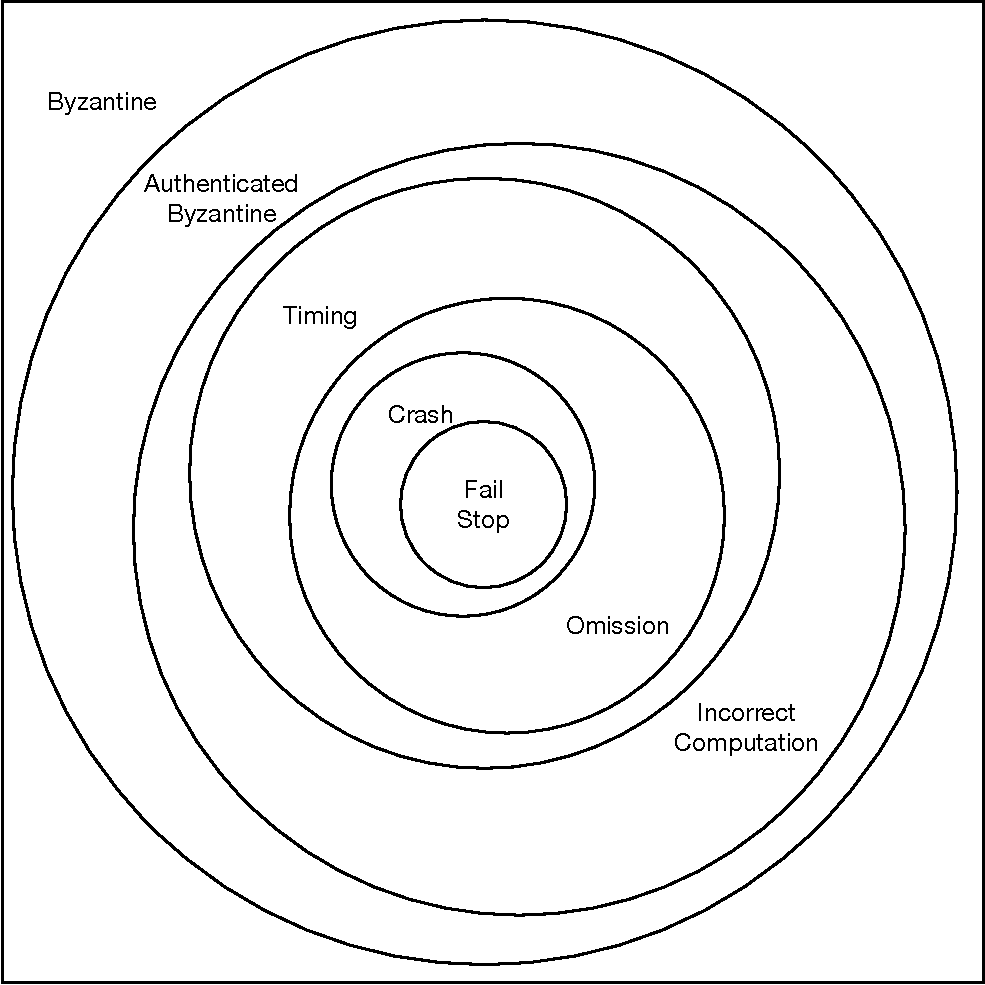
\includegraphics[width=0.5\textwidth]{img/AOFC.pdf}
  \caption{An ordered fault classification (Barborak et al.)}
  \label{fig:aofc}
\end{figure}

\subsubsection{Voting-Based Consensus Algorithm}
In order to vote the agreement, nodes of voting-based consensus algorithms have to 
know each other and be adjustable to communicate easier\cite{nguyen2018survey}.
Nodes communicate with others before making the decision 
to approve a proposed value or not.
Almost all the variants of voting-based algorithm contain the feature
that a majority of agreements is required to achieve the consensus.
However, since a node can crash, it brings the problem that the decision can not
be made through the majority's decision. Thus, at least \textit{f+1} nodes need 
to run properly when in the worst case \textit{f} nodes crash. 

Paxos\cite{lamport2001paxos} and Raft\cite{conf/usenix/OngaroO14} are 
crash fault tolerance based consensus.
Besides, Hyperledger Fabric\cite{cachin2016architecture} is 
Byzantine fault tolerance based consensus which 
uses Practical Byzantine Fault Tolerance\cite{castro1999practical}.
All of the three above are voting-based consensus algorithms.

\subsubsection{Proof-Based Consensus Algorithm}
The original work of proof-based consensus is called proof of work (PoW)
\cite{nakamoto2019bitcoin}. In PoW, nodes are only permitted to 
broadcast their proposal only when they have performed enough effort which
is usually done by computing power.
Unlike voting-based consensus which uses the majority's votes to 
make the decision on an agreement, proof-based consensus makes the decision 
following the decision of the node that performs sufficient proof.
When multiple nodes try to propose their own value, an agreement has to be made
by all the nodes. To achieve that, PoW gives a difficult puzzle with adjusted difficulty
and requires each node to solve it. The first node that solves the puzzle will make the
decision on an agreement and the others follow this decision.

There are many variants of proof-based consensus
which includes PoW, proof of sake (PoS), and their hybrod form. 
%% Maybe include in the future.
% \subsection{ACID Theorem}

\subsection{CAP Theorem and Consensus Algorithm} 
\label{sec:cap-theorem}

The CAP theorem \cite{brewer2012cap} states that, in a distributed system, it is impossible for an algorithm to provide more than two of these three properties:

\begin{itemize}
	\item \textbf{Consistency (C)}: All data backups in the distributed system have
    the same value at the same time.
	\item \textbf{Availability (A)}: After some nodes in the cluster fail, the entire
    cluster can still respond to client read and write requests. However, there
    is no guarantee that the data produced is most up-to-date.
	\item \textbf{Partition tolerance (P)}: The system continues to operate despite
    delayed, lost or dropped messages on the network.
\end{itemize}

Consensus algorithms like Paxos and Raft sacrifice availability to achieve partition-tolerance and consistency. Nodes in clusters that guarantee consensus can recover from partitions and maintain consistency, but the smaller part not in the majority partition (not in the quorum) will not send responses if partition problem happens. Hence the availability is compromised in consensus algorithms.

\subsection{Models of Computation} \label{sec:fundamental-models}

Solving the consensus problem varies in difficulty depending on the system model
being considered. Different models assert different assumptions and thus, it is
important to consider the impacts of such models on the consensus algorithms to
be investigated.

\subsubsection{Synchronous and Asynchronous Systems}

\textit{Fundamental models} provide an ``abstract perspective'' for considering
individual aspects of a distributed system \cite{coulouris2005distributed}. An
\textit{interaction model} is a fundamental model concerned with communication
and coordination between processes, including aspects such as process execution,
message delivery and clock drift \cite{coulouris2005distributed}. Although it is
difficult to set limits on these, considering ``two extremes of a spectrum''
gives rise to a pair of simple models---one with strong assumptions about time
and the other with none \cite{coulouris2005distributed, hadzilacos1994modular}.

The \textit{synchronous} system model is defined by Hadzilacos and Toueg
\cite{hadzilacos1994modular} to be one in which:

\begin{enumerate}
  \item Time taken by a process to execute a step has known upper and lower
    bounds.
  \item Every process has a local clock whose drift rate has a known bound.
  \item There is a known upper bound on message delay.
\end{enumerate}

These bounds are global across the entire system. A collection of processors
connected by a communication bus is an example of a system which closely aligns
to the synchronous model.

By contrast, the \textit{asynchronous} system model is one which makes no
assumptions about time \cite{coulouris2005distributed, hadzilacos1994modular}.
Namely, there are no bounds on process execution time or message transmission
delay and clock drift rates may be arbitrarily fast or slow
\cite{coulouris2005distributed}. This model is useful when considering systems
such as the Internet \cite{coulouris2005distributed}.

The asynchronous model is more general than the synchronous counterpart. As
such, it is more difficult to solve the consensus problem under the former than
the latter. An algorithm which works under the asynchronous model will also work
for the synchronous model.

The consensus problem is solvable under the synchronous model
\cite{fischer1985impossibility, kshemkalyani_singhal_2008}. However, it has been
shown by Fischer \cite{fischer1985impossibility} to be impossible to solve under
the asynchronous model. No matter the protocol or algorithm, there is always a
``window of vulnerability'' during which the failure of processes or delay of
messages prevents the system from reaching consensus by way of nontermination
\cite{fischer1985impossibility}. Despite this, it should be noted that the
impossibility arises from a worst-case scenario of low probability---in reality,
process scheduling has aspects of randomness \cite{aguilera2010stumbling}. Thus,
although it is not theoretically possible to guarantee consensus under the
asynchronous model in all circumstances, consensus algorithms can still be
implemented in practice.


\subsection{Relevant Problems} \label{sec:relevant-problems}

There are two other problems similar to the consensus problem---the
\textit{Byzantine generals problem} (also known as the \textit{Byzantine
agreement problem}) and the \textit{interactive consistency problem}. Table
\ref{tab:dbtap} provides a comparison between these and the consensus problem.
Despite the differences in requirements, a solution to any one of them can be
transformed to one of the others by reduction \cite{fischer1983consensus}.

\begin{table}[htp]
  \centering
  \begin{tabularx}{\linewidth}{%
    l%
    >{\raggedright\arraybackslash}X%
    >{\raggedright\arraybackslash}X%
    >{\raggedright\arraybackslash}X}
  \toprule
  Condition & Consensus & Byzantine Generals & Interactive Consistency \\
  \midrule
  \textbf{Termination} & Eventually decide on a \textit{value}
    & Eventually decide on a \textit{value}
    & Eventually decide on an \textit{array $A$} \\
  \addlinespace
  \textbf{Agreement} & Agree on the same value
    & Agree on the same value
    & Agree on the same array of values $A[v_{1} \ldots v_{n}]$ \\
  \addlinespace
  \textbf{Integrity}
    & The decided value is based on the propositions of all correct processes
    & If the commander is correct, then all correct processes decide on the
      value proposed by it
    & All correct processes decide on $v_{i}$ as the $i\textsuperscript{th}$
      component of their vector if $p_{i}$ is correct \\
  \bottomrule
\end{tabularx}
  \caption{Comparison of similar problems}
  \label{tab:dbtap}
\end{table}

The consensus problem is the key to many problems in distributed computing, 
making effective solutions to it highly desirable\cite{fritzke2001consensus}. To 
motivate consensus in context, related problems—highlighting useful applications 
in distributed computing—are discussed in this section. The following four 
issues are all related to consistency problem. They are reliable multicast, 
membership protocol (failure detector), leader election and mutual exclusion. 
The designer of distributed system should solve these problems primarily to 
ensure the stability and unity of the system.

\subsubsection{Reliable Multicast}

Reliable Multicast provide processes communication primitives so that they can 
broadcast and deliver messages in such a way that processes consistent not only 
on the set of messages they deliver but also on the order of message deliveries
\cite{fritzke2001consensus}. Usually, the problem of reliability is addressed by 
considering various types of reliability protocols. The problem of ordering 
properties are usually as follows.\cite{garcia1991ordered}

\begin{itemize}
  \item \textbf{Single source ordering}: If messages are from the same source 
  site, and they are sent to the same multicast group, then they should be 
  received by all target processes in the same order. 
  \item \textbf{Multiple source ordering}: If messages are from different 
  source sites, and they are sent to the same multicast group, 
  then they should be received by all target processes in the same order. 
  \item \textbf{Multiple group ordering}: If two messages are from different 
  source sites, and they are sent to different but overlapping multicast groups, 
  they should be received by all target processes in the same order.
\end{itemize}

Ordering in multicast is important, booking, banking, inventory and E-commerce 
are great applications built on distributed systems that require consistent 
message order between processes. In addition, ordered communication primitives 
can simplify the design of distributed application and reduce the possibility of 
related bugs due to synchronization or concurrency\cite{garcia1991ordered}. It 
is with these motivations that we will consider a reliable multicast technique 
when we choose consensus algorithms.

\subsubsection{Membership/Failure Detection}

Since it is impossible to safely distinguish between a crashed process and a 
slow process in an asynchronous distributed system, it is impossible to design 
a deterministic consensus algorithm in an asynchronous distributed system, even 
in the case of a single process crash failure\cite{fischer1985impossibility}. 
This impossibility prompted many researchers to propose a minimum set of 
assumptions. As long as these assumptions are satisfied by the asynchronous 
distributed system, the consensus problem can be solved as well. The unreliable 
fault detector gives the answer to this challenge\cite{chandra1996unreliable}. 

An unreliable failure detector consists of a set of oracles: every process has 
an oracle to provide a list of processes that are suspected to have crashed. 
racle will make mistakes, such as not suspecting a process that has crashed, or 
suspecting a process that has not crashed. When the oracle of the process 
p$_{i}$ suspects that p$_{j}$ crashed, we say that p$_{i}$ suspects p$_{j}$. 
The mistakes of the failure detector are typically defined by two properties:

\begin{itemize}
  \item \textbf{Completeness}: In the end, crashed processes should be 
  suspected. 
  \item \textbf{Accuracy}: Limit wrong suspicion of well-running processes. 
\end{itemize}

Chandra and Toueg\cite{chandra1996unreliable} defined several classes of failure 
detectors. One of them is named as $\diamond$S with following two properties:

\begin{itemize}
  \item \textbf{Strong completeness}: Ultimately, all crashed processes are 
  constantly suspected by every well-running process.
  \item \textbf{Eventual weak accuracy}: Ultimately, majority of well-running 
  processes are never suspected by any well-running processes.
\end{itemize}

In practice, if a process does not receive a message response before the timeout occurs, the message sending process suspects that the message receiving process has crashed. This can satisfy strong completeness. However, there is no guarantee of accurate process crash detection. In Raft and Paxos part, we will discuss how these two algorithm handle failure detection in detail respectively.

\subsubsection{Leader Election}

Leader election is to elect a leader in a group of processes and let all the processes of the group agree to the leader. A leader is the coordinator among processes and there can only be one leader at a time. In distributed system, each node must exchange messages with other nodes in the network to make a decision. However, this method of communication between nodes is time-consuming, and when consistency between all nodes is required, coordination between nodes becomes difficult. Therefore, choose a leader to manage the access of shared resources is necessary. The implementation of leader election should follow two basic properties\cite{nugraheni2009formal}:

\begin{itemize}
  \item \textbf{Safety}: There will never be two or more leaders at the same 
  time.
  \item \textbf{Liveness}: The election algorithm always ends, and each process 
  knows the leader who is ultimately elected.
\end{itemize}

In the leader election process, the leader is usually selected according to 
some criteria, such as the node with the largest identifier\cite{effatparvar2010improved}. After the leader is elected, the node will reach a state called termination state. There are two such states, namely the elected state and the non-elected state. When a node is in any state, it always maintains that state. Moreover, when the leader fails, the leader election mechanism can help to dynamically elect a new leader. Also in Raft and Paxos part, we will discuss how these two algorithm handle leader election in detail respectively.

\subsubsection{Mutual Exclusion}

The distributed mutual exclusion algorithm guarantees mutually exclusive access 
to a critical section among a number of competing 
processes\cite{lamport1987fast}. A mutual exclusion algorithm should meet the 
following principles\cite{velazques1993survey}: 

\begin{itemize}
  \item \textbf{}Only one process can be allowed to access its critical 
  section at the same time.
  \item \textbf{}If there is no process in the critical section, any 
  process asking an access to critical part must be allowed within a limited 
  time. 
  \item \textbf{}When a competing process request to access the critical 
  sections concurrently, it cannot be put off indefinitely.
  \item \textbf{}A requesting process cannot be prevented by another process 
  from entering critical section within a limited delay. 
\end{itemize}

In summary, an algorithm must provide mutually exclusive access to a resource, 
ensure the freedom of deadlock, ensure the freedom of starvation, and must 
provide a certain fairness in the order of granting requests. Mutually exclusive 
algorithms are divided into three categories:

\begin{itemize}
  \item \textbf{Token-based algorithm}: All processes share a token, and only the 
  process that obtains the token can enter the critical section. The safety, 
  liveness, and fairness of such algorithms are easily guaranteed. But there is 
  a disadvantage is that the token is lost, there is only one token in the 
  system, after the loss, you need to regenerate and ensure that the generated 
  token is still the only one in the system. 
  \item \textbf{Non-token-based algorithm}: Also called Permission-based. It is 
  through the exchange of messages between processes to determine whether they 
  can enter the critical section. 
  \item \textbf{Quorum-based algorithm}: The Quorum algorithm is actually a 
  Non-token-based algorithm, but the principle of the quorum algorithm is 
  different from other Non-token-based algorithms, so it is taken out 
  separately. The idea of Quorum is very simple, a collection of multiple 
  processes form a quorum, there are multiple quorum in the system, Any two 
  quorums will contain at least one common process, that is, the intersection 
  is not empty. Whether or not to enter the critical section depends on the 
  intersection process of quorum. 
\end{itemize}

\section{Comparative Analysis}
\label{sec:comparitive}
This section is based on the work \cite{howard2020paxos} which
presents the comparison between Paxos and Raft when they are 
both voting-based consensus. 
The comparison between voting-based consensus proof-based consensus consensus
is also shown in Figure~\ref{voting-proof}.
\begin{figure}[htp]
\begin{center}
\begin{tabular}{|c|c|c|}
\hline
\textbf{Criterion} & \textbf{Voting-based  Consensus} & \textbf{Proof-based Consensus} 
\\ \hline
Agreement making basement & \begin{tabular}[c]{@{}c@{}}From majority \\ of the node decisions\end{tabular} & \begin{tabular}[c]{@{}c@{}}Following nodes \\ performing enough proof\end{tabular} \\ \hline
Nodes can join freely & No & Mostly \\ \hline
Number of nodes executing & Limited & Mostly unlimited  \\ \hline
Decentralization & Low & Mostly high \\ \hline
Nodes identities are managed & Yes & No \\ \hline
\end{tabular}
 \caption{Comparison between Voting-based Consensus and Proof-based Consensus }
    \label{voting-proof}
\end{center}
\end{figure}

\subsection{Paxos and Raft}
Proof-based consensus algorithms are usually used for blockchains since its
original work is a peer-to-peer electronic cash system.
Because of difficult puzzles
are used, there is a high latency of making the decision on an agreement. 
Therefore this report only focuses on voting-based consensus. 
In the voting-based consensus, Paxos and Raft are the two dominate algorithms
\cite{howard2020paxos}.
Paxos is traditional and famous but also be known as difficult to understand.
Raft is a more recent proposed consensus algorithm and is more understandable
comparing with Paxos.

When Paxos and Raft are very similar to achieve distributed consensus,
the main difference between them is only in the leader election phase.
Paxos allows any node to become a leader and then updates its logs
if the new leader's log is not up-to-date. 
However, Raft only allows the node that with up-to-date logs to become the leader.
Therefore, there is no logs exchanging during leader election 
which makes Raft much more efficient than Paxos. 

State machines are both used in Paxos and Raft which compose a set of nodes 
to act as a single service that guarantees the consistency. 
The state machine requires the same order operations because 
programmers would treat the service as a single system even there are 
multiple nodes running in Paxos or Raft.

Raft achieve consensus in three different ways.
The first is the presentation. The Raft paper describes leader-based consensus 
using a new abstraction for state machine replication.
This new abstraction is popular with engineers.
The second is the simplicity. The Raft paper put simplicity at a higher priority but 
performance at the lower. For example, Paxos can append logs out-of-order 
although this requires extra protocols to filling the log in. 
Conversely, only in-order logs are allowed in Raft.
The third is underlying algorithm. The Raft algorithm uses a new approach to elect
the leader which makes not only leader election different 
but also the safety guaranteeing different.

\subsubsection{Approach}
Leader-based approach is many used in consensus algorithms including Paxos and Raft.
Those algorithms operate at a high level as follows:
One node is selected among all the nodes to be the \textit{leader}.
This leader asks the other nodes to append a same log, 
once the leader has received confirmation from a majority,
it then appends the logs to its state machine. This appending repeats in this leader until
its role changes or it fails.
When the repetition ends, a new leader will be elected from all the nodes.
Usually, at least a majority of votes are needed to elect a leader to 
ensure no overwriting happens on any previous logs.
\subsubsection{Basics}

\begin{figure}[htp]
\begin{center}
  \centering
  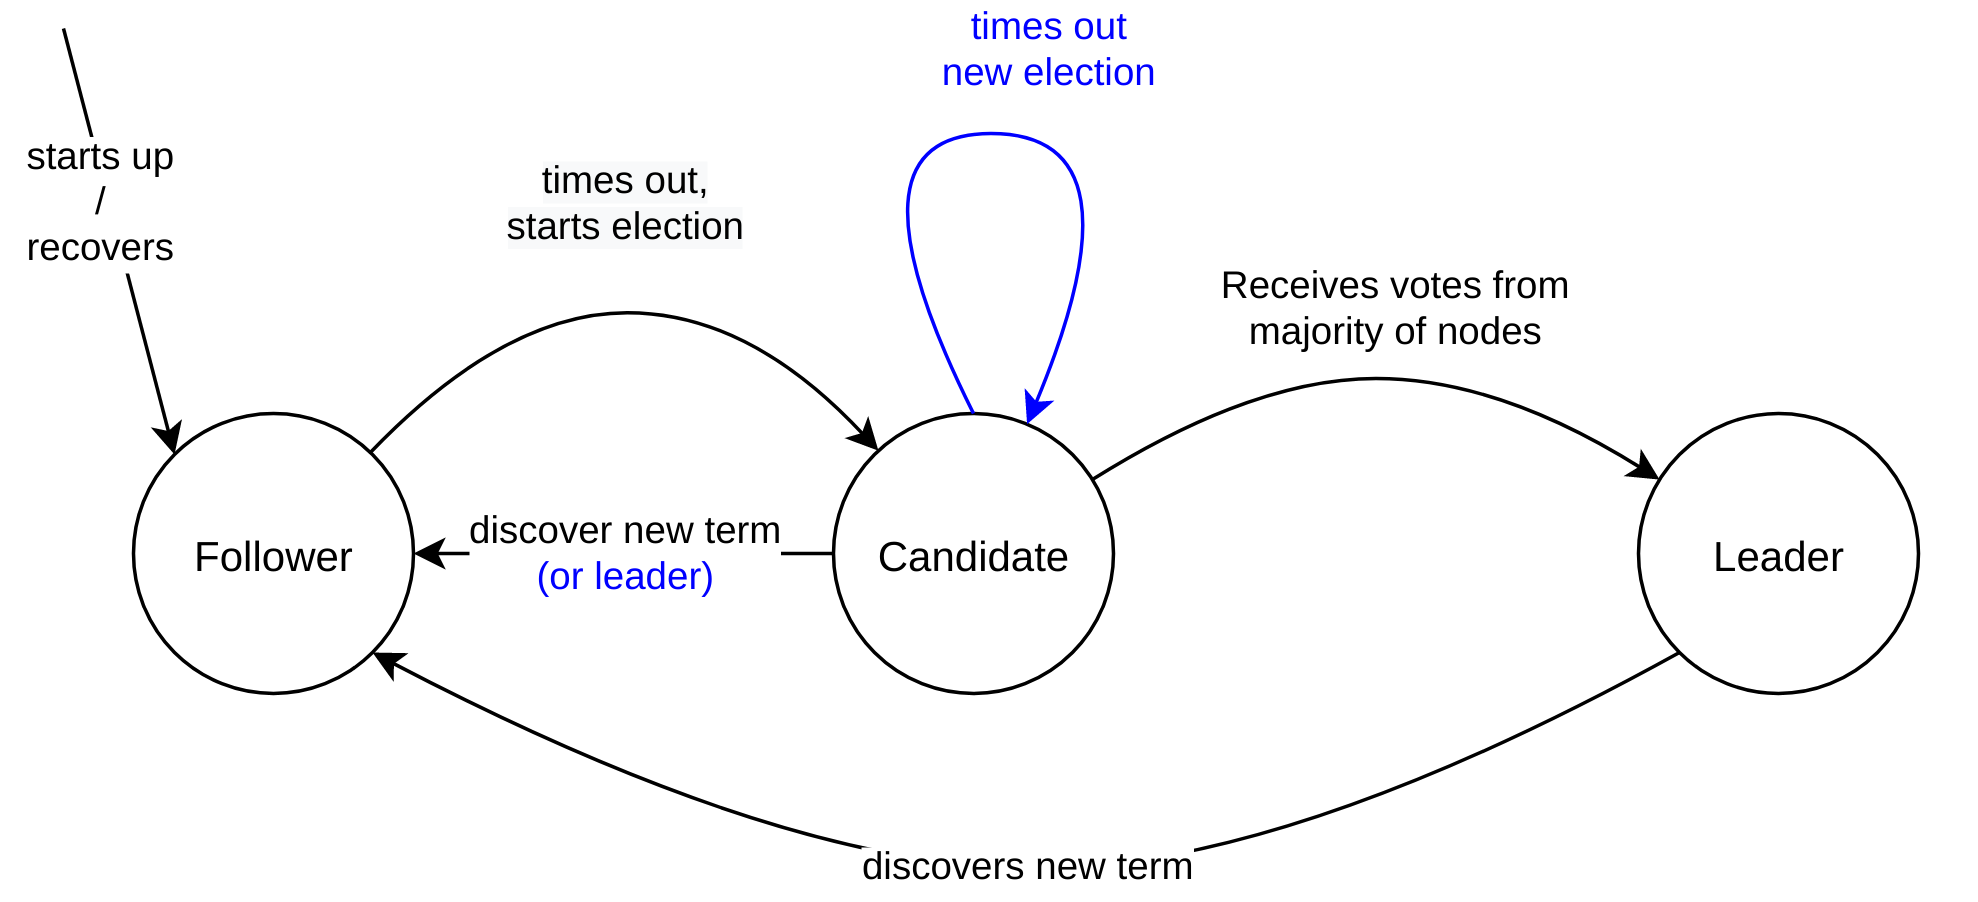
\includegraphics[width=0.8\textwidth]{img/roles-transitions.png}
  \caption{Role transitions between the nodes for Paxos \& Raft. The blue transitions are for Raft only.}
  \label{fig:roles-transitions}
\end{center}
\end{figure}
As Figure~\ref{fig:roles-transitions} indicates, a node may be a \textit{Follower}, 
a \textit{Candidate} or a \textit{Leader}. 
The \textit{Follower} is responsible for
remote procedure calls which also includes voting for a leader.
The \textit{Candidate} is only at the election phase when a node in \textit{Candidate}
is trying to become a leader.
The \textit{Leader} is responsible for appending logs to its state machine after
asked other nodes to do it.

At the very beginning, all nodes are follower. Each of the nodes keeps its follower role 
until it believes the leader has failed, then it becomes a candidate trying to become
a leader. If a node successfully became a leader, the others became followers following
the appending operation broadcasted by this leader.
Each nodes also keeps a number, named \textit{term} which used to perform leader election
during the running time of the whole system. When a node receives any message,
it firstly check the term of the sender, if the sender's term is greater than local term,
the node updates its term using the greater one and then reacts according to the message. 
If the two terms are equal, the node reacts directly. Otherwise, if the sender's term
is smaller than the local term, it responds to the sender with its greater term and change
itself to be a candidate trying to become a leader.

\subsubsection{Log Entry}
A log entry is a pair of operation an term. Operations are sent to the leader 
in log entries from followers. The leader is responsible for receiving the log entries and
maintaining the consistency of the whole system. 
When the leader receives a log entry, the leader asks followers to append the log entry,
if a majority of followers responds that with the confirmation of the appending,
the leader then records the very operation to its state machine.
To make the logs in order, in this phase, a follower can only append a log when 
its prior log or logs are identical to the leader's log. And a follower can only 
respond its confirmation after it recorded the appending to its state machine.

\subsubsection{Leader Failures Handling}
Despite of the previous similar points for Paxos and Raft, they have different
strategies to handle leader failures.

For Paxos, a follower becomes a candidate if it failed to receive any message
from the leader for a specific time. 
The term of it will be increased to the next such that 
\textit{term mod n = s} where \textit{term} is the next term, 
\textit{n} is the count of nodes and \textit{s} is the node id of this candidate. 
During this election, this candidate has to make sure it has all the previous logs
before it becomes a leader. Thus, followers that vote for this candidate should respond
with a election message which also includes all the log entries that the follower
has after the candidate’s commit index.
The candidate reviews all the log entries it received, compares them with its own logs.
If the candidate has a same log, it updates its own log with the new term.
If the same index has multiple log entries , the candidate uses the 
greatest and newest term to update the conflict log.
After all log entries checked, the candidate then can become a leader
and starts to replicate the log entries to followers.

For Raft, a node will also become a candidate and It increases its term if it failed to receive any message
from the leader for a specific time. 

\subsubsection{Summary}
Overall, Raft is easier to understand and implement, which makes it more commonly used. But in essence, the approach of Paxos and Raft is quite similar, the only difference between them is that the process of election of the leader of raft is simpler. Specifically: (i) When choosing a leader, Paxos divides terms between servers. While in raft, each follower can be a candidate in any term, but each follower can only vote for one candidate, and the candidate with the majority votes will become the leader. (ii) 





\section{Paxos Algorithm} \label{sec:paxos}

Draft: What Paxos do we have?

Paxos \cite{lamport2001paxos}, Fast Paxos \cite{fastpaxos}, 
S-Paxos \cite{spaxos}, 
OpenReplica \cite{openreplica} and Ring Paxos \cite{ringpaxos}.

\begin{figure}[htp]
  \centering
  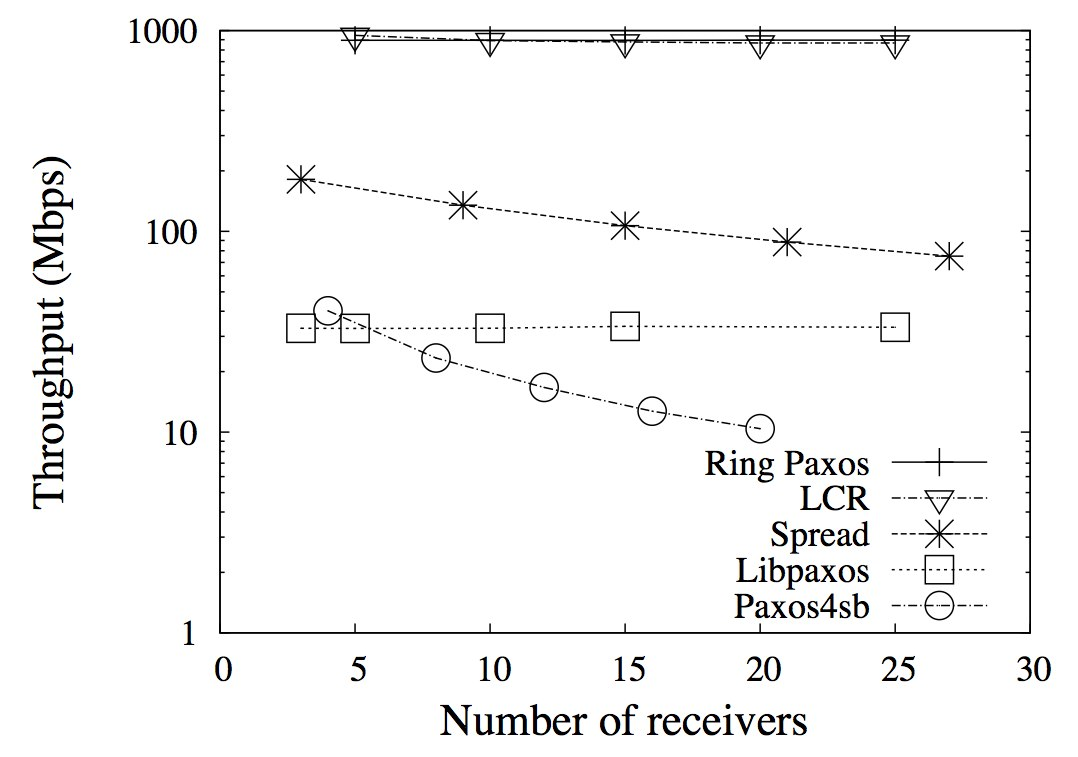
\includegraphics[width=0.8\textwidth]{img/RingPaxosThroughput.jpg}
  \caption{Ring Paxos Throughput}
  \label{fig:RingPaxosThroughput}
\end{figure}


\subsection{Problem}
In distributed computing, there are processes cooperating with each other. 
Paxos is designed to achieve consensus which ensures 
only a single value is chosen from proposed values that 
proposed by some processes\cite{fischer1983consensus}. 
After been chosen, this value is also available to be learnt by all processes
when a process can only learn a value that has been chosen.


The following content of this section explains 
Paxos algorithm based on \cite{fischer1983consensus}. 
In their work, they make two assumptions, 
based on that, they then give principles to solve the consensus problem. 
These principles require a proposing approach 
of which each proposal has an ordered number \textit{n} 
and a proposal value \textit{v}. 
The principles also require three classes of agents 
which are proposers, acceptors and learners. 
There are two phases when choosing a value.
\textit{Phase1} is to \textit{prepare} a proposal 
by requesting a majority of acceptors. 
\textit{Phase2} is to ask the majority to \textit{accept} this proposal.
In this phase, any acceptor among the majority can 
either accept or decline the \textit{accept} request.

\subsection{Two Assumptions}
\begin{quote}
  \begin{assumption}{1}{F}\label{as:1}
    Processes run asynchronously. 
    They may have arbitrary running speed, may fail and may restart.
  \end{assumption}
  \begin{assumption}{2}{F}\label{as:2}
    Processes can communicate with each other by message passing. 
    Messages can take arbitrarily long to be delivered. 
    Messages can be duplicated, can be lost, but can not be corrupted.
  \end{assumption}
\end{quote}
\subsection{Two Principles}

The principles are given here and will be applied later,
\begin{quote}
  P1. An acceptor must accept the first proposal that it receives.
  \begin{quote}
    a. An acceptor can accept a proposal numbered \textit{n} 
      iff it has not responded to a \textit{prepare} request 
      having a number greater than \textit{n}.
  \end{quote}
  P2. If a proposal with value \textit{v} is chosen, 
    then every higher-numbered proposal that is chosen has value \textit{v}
    \begin{quote}
      a. If a proposal with value \textit{v} is chosen, 
        then every higher-numbered proposal accepted 
        by any acceptor has value \textit{v}.
        
      b. If a proposal with value \textit{v} is chosen, 
        then every higher-numbered proposal issued 
        by any proposer has value \textit{v}.

      c. For any \textit{v} and \textit{n}, 
        if a proposal with value \textit{v} 
        and number \textit{n} is issued,
        then there is a set \textit{S} consisting of 
        a majority of acceptors such that either 
          \begin{quote}
            (i) no acceptor in \textit{S} has accepted 
              any proposal numbered less than n, or 
              
            (ii) \textit{v} is the value of 
              the highest-numbered proposal among 
              all proposals numbered less than 
              \textit{n} accepted by the acceptors in \textit{S}.
          \end{quote}
  \end{quote}
\end{quote}

\subsection{Three Agents}

To achieve the consensus, there are three classes of agents 
which are proposers, acceptors and learners. 
When a process proposes a proposal, 
it is included in the class of proposers.
When a process receive requests from any of the proposers,
it is then included in the class of acceptors.
And when a process learn a chosen value, 
it is included in the class of learners.
These three cases can happen simultaneously, i.e.
a process can propose, receive requests or 
learn a chosen value at the same time.
Thus the three classes of agents are 
not mutually exclusive for a single process.


\subsection{Implementation}
\subsubsection{Choosing A Value}\label{Choosing}
The Paxos algorithm \cite{lamport1998part} chooses a leader 
from the processes of assumption \ref{as:2}. 
This leader is the leader of the class of proposers and 
also the leader of the class of learners at the same time. 
A proposal is tagged with an ordered number \textit{n} and a value \textit{v}.
The proposal will be passed from one proposer to the leader. 
This leader is in charge of requesting a majority of accepters to ask for 
acceptance.
The majority can be generated by the algorithm \cite{keidar2001cost}.
A proposal will be requested two times to finally be chosen.
At the first time request, named \textit{prepare} request, 
an acceptor should respond the proposer leader with a \textit{promise} respond.
Once get \textit{promise} respond from a majority 
(this majority could be different from the requested one),
the proposer leader requests each \textit{promised} acceptor 
in the majority with an \textit{accept} request 
to confirm the acceptance of this proposal.
The acceptor which receives this \textit{accept} request 
will accept this proposal based on $P1^a$. 
And no matter it accepts it or not, it should respond the proposer leader to
confirm their reaction.
If a proposal was proposed, i.e. a value was chosen, 
then it comes to learn it.

\subsubsection{Learning A Value}
There are three easy approaches to learn a value.
The first, in \textit{Phase2}, when acceptors accept a value, 
they can respond to all the learners. 
This is immediate but requires a response number at
the product of the number of learners and the number of acceptors.
The second, accepters now respond only the leader of learners. 
However, this is unreliable since we have the assumption\ref{as:2}.
It brings us to the third way, which is to have a set of leaders of learners
combining the benefits of the other approaches without lots of message passing.

The three ways above are all passive in the perspective of a learner when
it is actually be notified what the chosen value is.
If a learner want a chosen value itself, 
it can get an another agent to be  a proposer 
to propose a proposal using the above algorithm. 
\subsection{Protocol}
\cite{PaxosMadeSwitch-y} uses UDP to pass messages, 
they think Paxos does not require reliable communications, 
so using TCP is unnecessary.
\subsection{Issues}
Because of assumption\ref{as:1} and 
the use of a quorum of acceptors \cite{jalili2014practical}, 
with that acceptors handling messages sequentially,
performance hiccups may occurs when it takes time for slower acceptors 
to catch up.


Paxos has several significant shortcomings. The first one is that it 
is exceptionally difficult to understand\cite{conf/usenix/OngaroO14}. 
To describe the Paxos algorithm, Lamport described a parliament on a 
small island in Greece\cite{lamport1998part}. The original paper is 
very vague and few people can fully understand it. Although Lamport 
later published a paper trying to simplify the description of the 
algorithm\cite{lamport2001paxos}, understanding Paxos is still a big 
challenge. Another drawback of Paxos is that it does not provide a 
good foundation for building practical implementations\cite{conf/usenix/OngaroO14}.
The description of the algorithm in Lamport's paper is just an 
algorithm for a single decree. Lamport mentioned the solution to 
implement Multi-Paxos, but many details are not sufficiently provided, 
which leads to the existing implementation of Paxos based on the 
implementer's own understanding. As a result, practical systems usually
vary widely.

\subsection{Optimisations}
To prevent failures described in assumption\ref{as:1}, 
stable storage is used by both proposers and acceptors.
The highest-numbered proposal is always stored in a proposer's stable storage.
The intended response is always stored in an acceptor's stable storage
before it responds.

\section{Raft algorithm} \label{sec:raft}
The Raft algorithm was proposed in 2014\cite{conf/usenix/OngaroO14} as an alternative to the (Multi-)Paxos algorithm, which is more
understandable and easier to implement a practical system. The highlight of the Raft algorithm is that it adopts an
engineering thinking --- It simplifies the model of the design according to the requirements in practical applications and
modularizes the process of the algorithm. From the perspective of performance and security, the Raft algorithm is also almost
the same as Paxos \cite{conf/usenix/OngaroO14}.
\subsection{Roles}
  \subsubsection{Follower}
  All nodes are followers when they are started. The followers are completely passive, they can only respond to incoming
  messages. If the client's message is sent to a follower, the message will be redirected to the leader of this cluster. Followers may
  also be able to become a leader through elections under certain conditions.
  \subsubsection{Leader}
  There can be only one Leader in the entire cluster at the same time. The leader handles all client interactions.
  \subsubsection{Candidate}
  The candidate state is a state between the follower state and the leader state. When a follower becomes a candidate, an election
  will be held. The candidate who wins the election will be the new leader.
  \begin{figure}[htp]
      \centering
      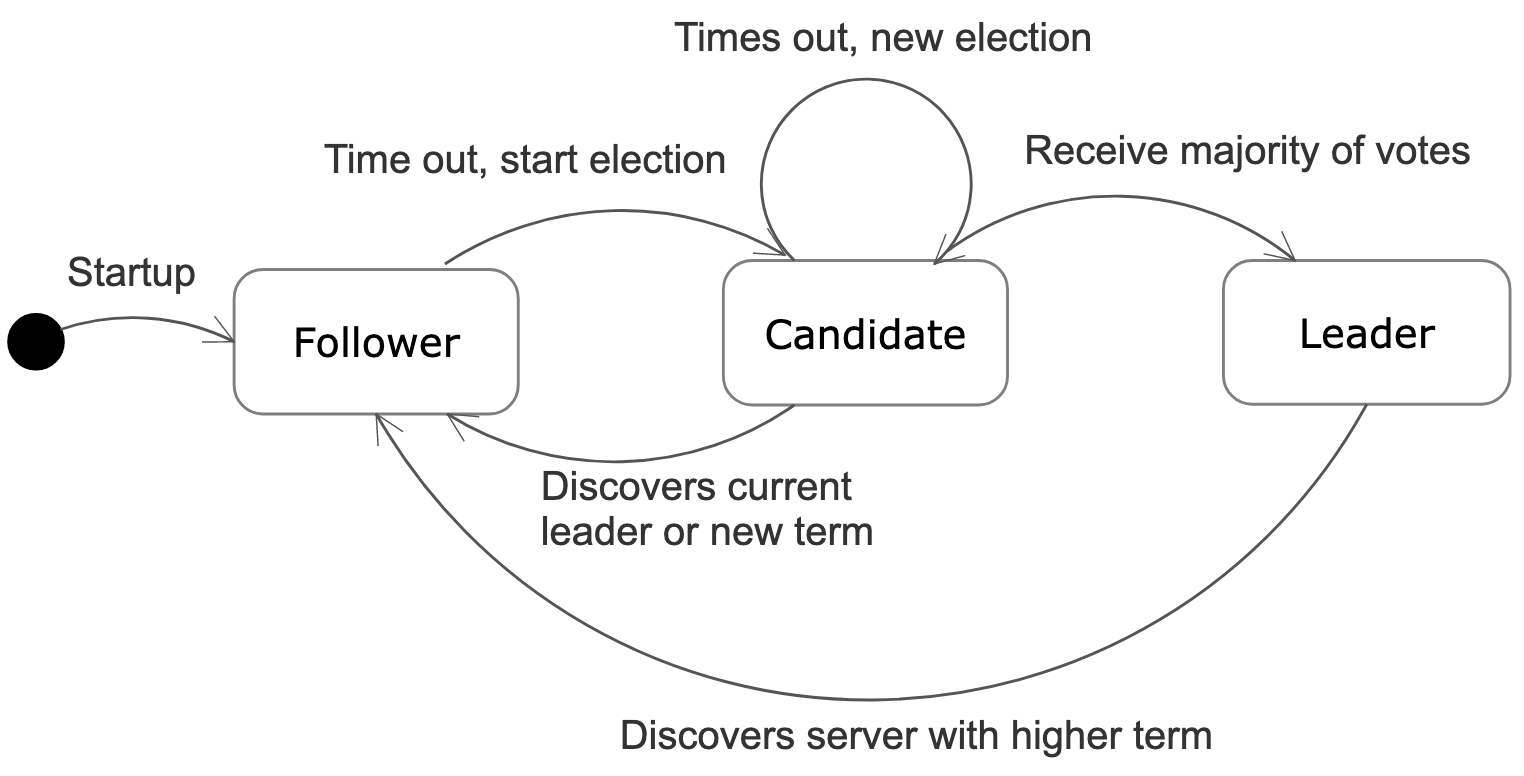
\includegraphics[width=0.8\textwidth]{img/raft-state-diagram.png}
      \caption{Server states}
      \label{fig:aofc}
  \end{figure}
\subsection{Protocol}
In the Raft algorithm, time is divided into terms\cite{conf/usenix/OngaroO14}, Each term has a number, and the number increments when a new term starts. Each term starts
with an election. If the election is successful, then the chosen leader will serve out for the rest of the term, which means that
only one leader can be elected in a given term. If the election is not successful, then the candidate starts a new term. Each node
in the cluster maintains the value of the current term number and it should be stored reliably. The function of the term and term number is
to allow the nodes to identify the information that is out of date.
\par
In order to let the followers believe there is an active leader in the cluster, followers expect to receive heartbeat messages from
the leader regularly. If the follower's timeout of heartbeat message elapses, it assumes that the leader crashed and will start a
new election. This timeout is often much longer than the propagation time of the message in the network.
\par
There are only two type of RPCs in the Raft algorithm:
\begin{itemize}
  \item \textbf{RequestVote RPC}: invoked by candidates to gather votes\cite{conf/usenix/OngaroO14} from other nodes.
  \item \textbf{AppendEntries RPC}: invoked by the leader to replicate log entries\cite{conf/usenix/OngaroO14}.
\end{itemize}
  \subsubsection{Leader Election}
  When a node begins an election, the first thing it does is to increment its current term number. The node then converts itself from
  follower state to candidate state. To win the election, the node must receive votes from a majority of nodes in the cluster. The node
  votes for itself, then send RequestVote RPCs to all other nodes and retry this process until:
  \begin{itemize}
    \item It receives votes from majority of nodes in the cluster, which means it wins the election and becomes the leader.
    \item It receives a RPC from a leader, which means one of other candidates wins the election, the current node becomes a follower.
    \item Election timeout elapses, which means no one wins the election. The node will then increment the term number and start a new election
  \end{itemize}
  \par
  To ensure safety, each node can only give out at most one vote in a term. This guarantees that only one candidate can get votes from
  the majority in the same term, thus only one candidate can win the election. Also, to prevent live lock of the election, the election
  timeout of each node is chosen randomly.
  \subsubsection{Log Replication}
  Once a leader is elected, it receives all client's request messages. These messages contain a command to be executed by the replicated
  state machine. The leader creates a log entry for each request from the clients. Apart from commands, the log entry also contains an index
  number in the log and a term number when the log entry was first created. Each log entry is committed if known to be stored in the logs of
  the majority of the nodes.
  \par
  When the leader receives a command from a client, it appends the command with the current term number and index number to its log. Then the leader
  sends AppendEntries RPCs to all followers. Once a new log entry is committed, the leader passes the command to its state machine and
  notifies all followers of this new log entry. When the followers receive these RPCs, they pass the command to their state machine.
  \par
  To ensure consistency of logs, each AppendEntries RPC contains the index and the term of the previous log entry. The followers who receives the RPC will
  reject the request if they do not have a matching log entry. It then is guaranteed that a new entry is only accepted if the logs match in
  their previous entry. So if a given log entry is committed, its all previous log entries are also committed.
  \par
  At the beginning of a new leader's term, the old leaders may have left some log entries that are partially replicated. The way that the Raft
  algorithm used to solve this problem is to force all follower to duplicate its log, which will also force all follower to discard all the
  inconsistent log entries and fill in all missing log entries. The leader maintains a value nextIndex for each follower, which marks the index
  of the next log entry to send to that follower. When AppendEntries consistency check fails, it decrements the nextIndex and retries until the
  follower's log is repaired.
  \subsubsection{Safety}
  If a leader has decided that a log entry is committed, then that entry should be present in the logs of all future leaders\cite{conf/usenix/OngaroO14}. To guarantee this,
  the algorithm picks the candidate to win the election such that it has the log that is most likely to have all the entries that have been
  committed. So the candidates must include log info in RequestVote RPCs including index and term of the last log entry. And the voting servers
  have to deny if its log is more complete.
  \par
  Another safety issue is that if a leader crashes while replicating logs, the new leader will not know whether the last log entry of the
  previous leader has been committed or not. To solve this problem, a new commitment rule must apply --- For a leader to decide an entry
  is committed, in addition to the previous rule, at least one new entry from leader's term must also be stored on the majority of servers.

\section{Application} \label{sec:application}
We implement a distributed key-value database using the Raft consensus algorithm. Although Paxos is the dominant consensus algorithm in the industry, Raft is selected due to its strong focus on being an understandable algorithm. Further, unlike Paxos, Raft is a \textit{continuous} algorithm which we deem to be more suitable for our application. Although there is a variant of Paxos which is similarly continuous (Multi-Paxos), we find the Raft algorithm to be less complex to implement. 

Our key-value database takes the form of a \texttt{HashMap} which is replicated (as opposed to sharded) across all nodes in the cluster. Due to this replication, it is crucial that our system remain consistent over time; key-value pairs should match across different nodes. Hence, we solve the problem with the aid of consensus.

\subsection{Architecture}
All nodes in our system share the same architecture, shown in Figure \ref{fig:aofc}. Below, we discuss the rationale behind our design decisions.

\texttt{NodeImpl} is the main class of a node, holding references to a \texttt{RaftLog} object and an object corresponding to the current state of the node (i.e. follower, candidate or leader). The class implements \texttt{INode} (which extends \texttt{Remote}) to be able to receive RMI calls from other nodes---the \texttt{requestVote} method is called by candidate nodes and the \texttt{appendEntries} method is called by the leader. Additionally, the class implements \texttt{IClientInterface} to be able to receive RMI calls from clients.

However, \texttt{NodeImpl} does not hold a direct reference to the \texttt{StateMachine} object. Instead, the reference to the state machine (which contains the \texttt{HashMap} with the state of the key-value database) is held by the \texttt{RaftLog} object instead. This design decision was made as a safeguard against system inconsistencies which could possibly arise from unintentional manipulation of the state machine. \texttt{NodeImpl} should not concern itself with the state machine; its focus should rather be on appending and committing \textit{log entries}. The \texttt{RaftLog} object takes responsibility for applying the correct log entries to the state machine, based on whether they have been successfully committed.

The three different states in which a node can be correspond to three classes---\texttt{CandidateState}, \texttt{FollowerState} and \texttt{LeaderState})---to segregate behavioural differences based on state and avoid the need to repeatedly check the state that the node is in. These classes all extend \texttt{AbstractState} which encapsulates common parameters such as the minimium and maximum election timeout.

We made a conscious decision to make attributes of \texttt{AbstractState} such as \texttt{currentTerm} and \texttt{votedFor} static. Since the application is distributed, all nodes run on separate machines (and hence, different JVMs). Thus, there is no issue with making these attributes static. By doing so, we have the benefit of the values being carried over seamlessly when a node changes state; the attributes are not tied to a specific object.

\begin{figure}[htp]
  \centering
  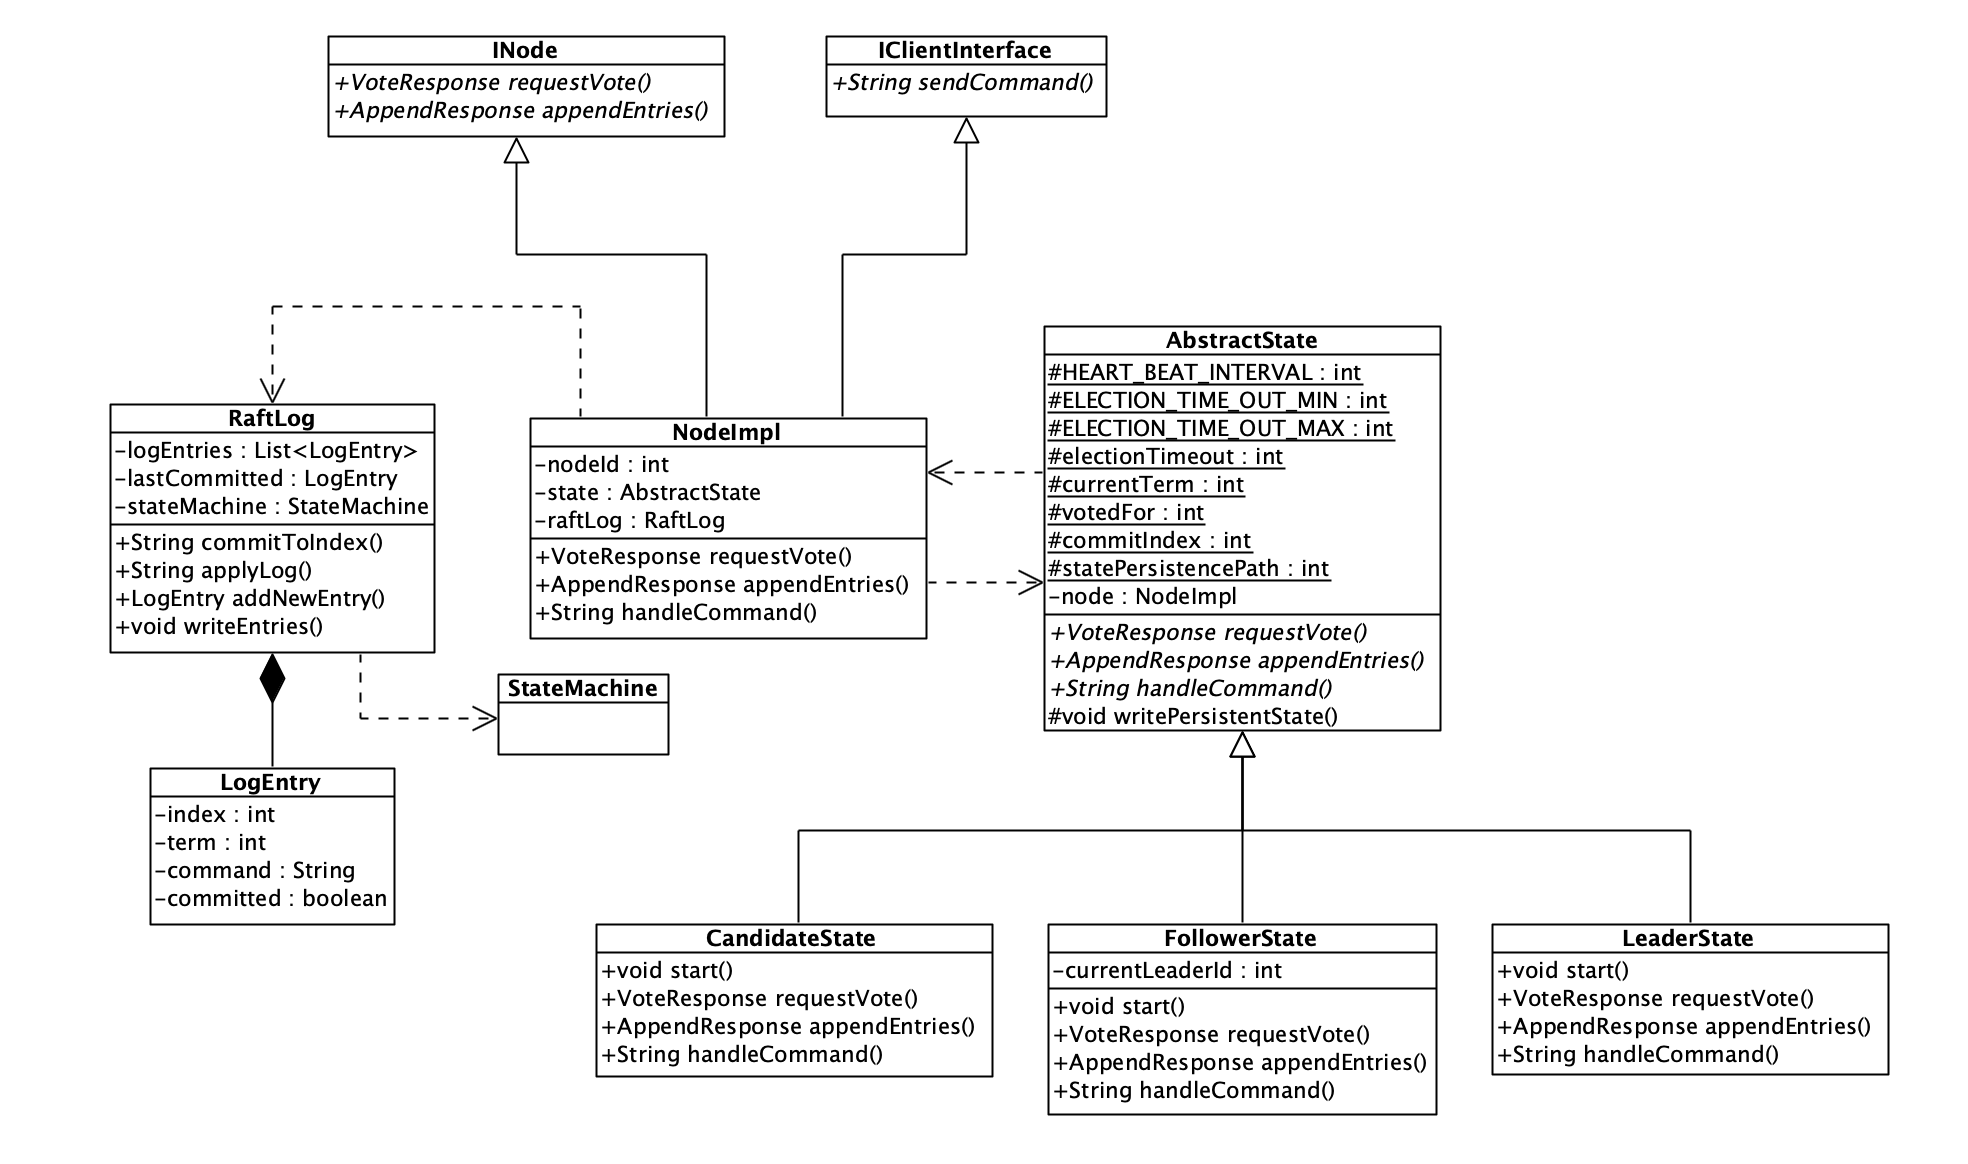
\includegraphics[width=1\textwidth]{img/class-diragram.png}
  \caption{Class Diagram}
  \label{fig:aofc}
\end{figure}

\subsection{Operation}
The system is made available by starting at least half the nodes in the cluster. All nodes have a configuration file detailing:
\begin{itemize}
    \item The ID of the node
    \item For every other node in the cluster:
    \begin{itemize}
        \item Its ID
        \item Its IP address and port
    \end{itemize}
\end{itemize}
Upon starting a node, it attempts to connect to all other nodes listed in the configuration file. In the event that it can't connect to a particular node, it tries again periodically for up to 30 seconds before continuing to the normal state of operation. As per the Raft algorithm specification, all nodes start in the follower state. The transition from one state to another is handled by the incumbent state. For instance, should a leader node receive an \texttt{appendEntries} RMI call containing a higher term than its own, its \texttt{state} object (i.e. \texttt{LeaderState} object) will handle cleanup operations (such as ensuring that periodic heartbeats no longer be sent) and instantiate a new \texttt{FollowerState} object, reassigning the \texttt{state} attribute of the \texttt{NodeImpl} object to the newly created object.

During operation, changes made to the log are written to persistent storage. This ensures that upon crashing and recovering, a node can simply read the previous state of the log. Note, however, that this is not a requirement of the algorithm. Indeed, a node in our system can recover successfully even if all previous log entries are lost (e.g. due to storage corruption). Nonetheless, recovery is made more efficient if the log is written to persistent storage, since fewer log entries need to be sent from the leader in order for the recovered node's log to catch up.

\subsection{Advantages and Disadvantages}


\bibliographystyle{ieeetr}
\bibliography{main}

\end{document}
